
\paragraph{Variaci\'on de la \textit{sparcity}}
Al variar la relaci\'on de cantidad de links frente al tama\~no de la matriz, estamos cambiando que tan rala es la matriz. Para analizar esto,
tomamos en cuenta la \textit{sparcity} la cual representaremos de ahora en m\'as como $\delta = 1 - \frac{n}{m^2}$. A continuaci\'on se muestra 
el gr\'afico obtenido a partir de la experimentiaci\'on dejando fijos $n = 100$, $p = 0.8$, $\varepsilon = 10^{-5}$ y variando $m$ desde $100$
hasta $8000$ de a $100$.
\begin{figure}[H] 
\centering
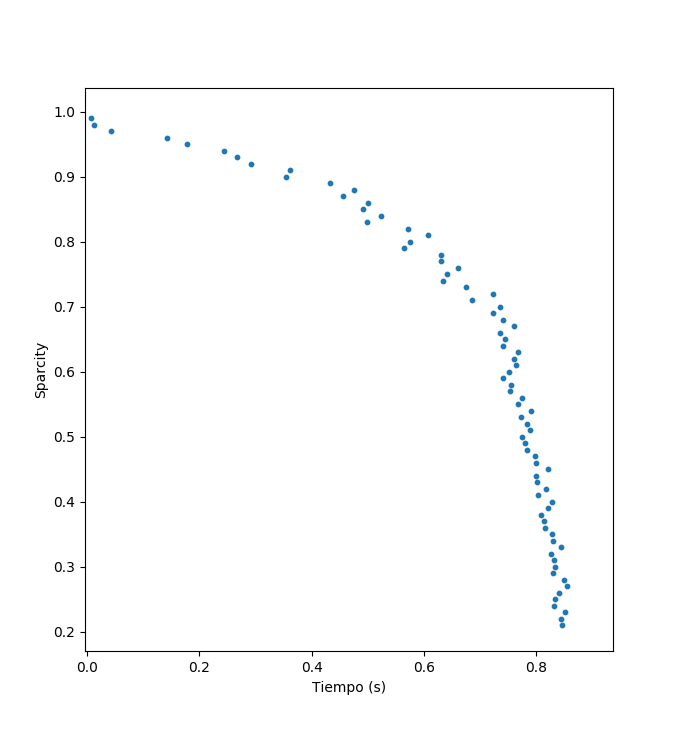
\includegraphics[width=0.7\textwidth]{img/sparcity.png}
\caption{Gr\'afico de sparcity en funci\'on del tiempo}
\label{fig:sparcity}
\end{figure}
A partir de este gr\'afico podemos observar como, tal como fue predicho, que a medida que la matriz es menos rala ($\delta \approx 0$) aumenta
considerablemente el tiempo que demora en ejecutarse el algoritmo.


\paragraph{Variaci\'on de la probabilidad}
Para analizar la incidencia de la probabilidad en el tiempo requerido, tomamos como par\'ametros fijos $n = 1000$, $m$ = 500,
$\varepsilon = 10^{-5}$ y variamos $p$ desde $0.01$ hasta $0.99$ con un incremeto de $0.01$ en cada paso.
\begin{figure}[H] 
\centering
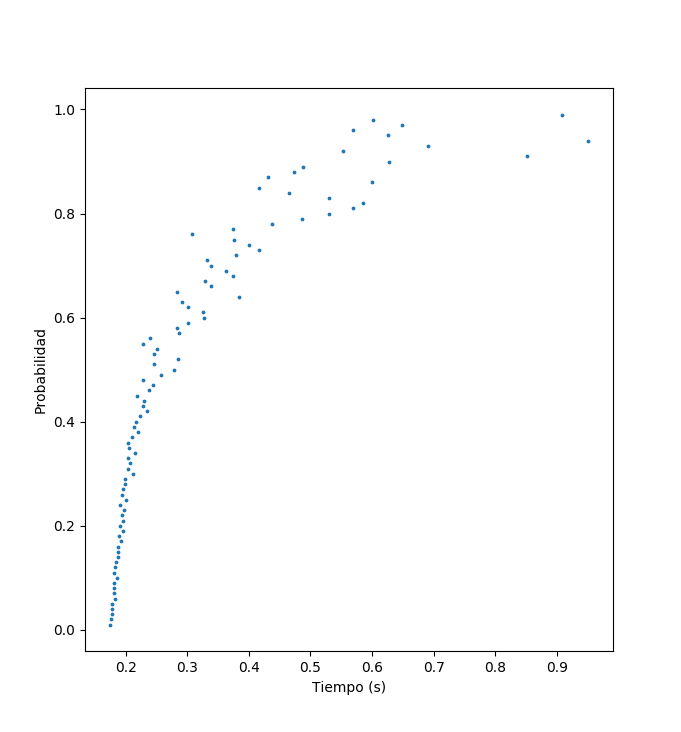
\includegraphics[width=0.7\textwidth]{img/Proba.png}
\caption{Gr\'afico de probabilidad en funci\'on del tiempo}
\label{fig:proba}
\end{figure}

Se puede apreciar como la elecci\'on de la probabilidad tambi\'en afecta en el tiempo de ejecuc\'on, tal como nos im\'aginabamos previo al experimento.

\paragraph{Variaci\'on del epsilon}

Para analizar c\'omo afecta el $\varepsilon$ con el tiempo, tomamos como par\'ametros fijos $n = 1000$, $m$ = 500,
$\varepsilon = 10^{-5}$ y variamos $p$ desde $0.01$ hasta $0.99$ con un incremento de $0.01$ en cada paso.
\begin{figure}[H] 
\centering
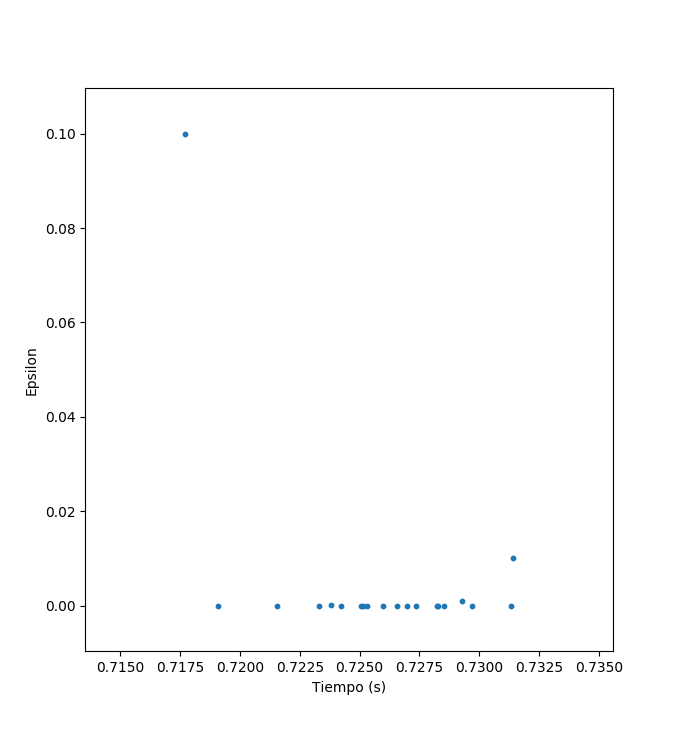
\includegraphics[width=0.7\textwidth]{img/Eps.png}
\caption{Gr\'afico de epsilon en funci\'on del tiempo}
\label{fig:eps}
\end{figure}

En este caso, pese a correr varias veces el test con distintos valores, no logramos apreciar correlaci\'on alguna entre la variaci\'on del $\varepsilon$ y el
tiempo.

\paragraph{Tests cualitativos}

Para armar nuestros experimentos, tomamos un p = 0.80, un valor cercano al de los casos dados por la c\'atedra. Y si bien los casos pr\'acticos del rankeador se presentan con un n mucho mayor, elegimos 25, una cantidad de p\'aginas acotada para que nuestro ejemplo no deje de ser facilmente comprensible.

Links entrantes: En este grafo hay dos nodos en los cuales se concentran muchos links entrantes de cada subgrafo, estos dos nodos tienen cada uno un link que apunta al mismo nodo, este a su vez, retroalimenta el ciclo, apuntando a los nodos mas bajos de la cadena.
En este caso esperamos ver que los nodos mas pesados del grafo sean aquellos que reciben muchos links entrantes, y el nodo al que apuntan los dos previamente mencionados.

Resultado: El nodo que tiene las dos entradas resulta ser el mas importante, y los dos nodos con muchas entradas son los segundos m\'as importantes. 

Links salientes: Este grafo es similar al anterior, pero los links tienen las direcciones invertidas, por lo tanto, en este grafo los nodos con muchos salientes terminan concentrando su peso en el nodo que retroalimenta el ciclo apuntando a los dos nodos con muchos links salientes.
En este experimento esperamos que el nodo con mayor probabilidad sea el que retroalimenta el ciclo, y que los nodos a los que esto apunta sean los siguientes con mayor probabilidad.

Resultado: El nodo que concentra todos los caminos y retroalimenta el ciclo resulta ser el nodo mas importante del grafo, seguido por los nodos con muchos links salientes, y a medida que se avanza en el ciclo, las probabilidades van bajando.

Links grafos separados: En este caso, hay 3 subgrafos sin conexi\'on entre ellos, no hay ning\'un tipo de estancamiento, es decir, todos los nodos tienen links salientes.

En este experimento esperamos que los nodos con m\'as probabilidad sean aquellos que reciben el \'unico link saliente de otro nodo, o aquellos que sean un paso obligado para unir dos partes distintas de cada subgrafo.

Resultado: Los nodos mas probables resultaron ser aquellos que adem\'as de recibir el \'unico link saliente de otro nodo y ser un paso obligado, tienen un ciclo con otro nodo.

Links a ciclo: En este grafo hay un grupo de grafos que permanece ciclando, y otros, que se relacionan entre ellos, apuntando finalmente a un nodo que sirve de nexo entre los dos grupos.

El resultado esperado en este caso es que los nodos del ciclo tengan mayor peso que los dem\'as nodos.

Resultado: Los nodos m\'as probables en este caso resultaron ser los nodos del ciclo y tambi\'en el nodo que conecta las dos partes del grafo.

Links a ciclo al rev\'es: En este caso, hay dos mitades del grafo, una con ciclos y otra con dos nodos sin links salientes que sirven como final para la mayor\'ia de caminos posibles, dichas partes est\'an conectadas por un \'unico nodo.

En este caso esperamos que los nodos que sirven como final sean de los m\'as probables, tambi\'en que los nodos que ciclan y el nodo nexo lo sean.

Resultado: Debido a la diferencia de caminos, uno de los nodos finales se impuso como m\'as probable, seguido por los nodos pertenecientes al ciclo, luego de estos, el otro nodo final y el nodo nexo.


En las figuras \ref{fig:Ranking cadena simple}, \ref{fig:Ranking cadena con nodo central}, \ref{fig:Ranking nodos con muchos links salientes} y \ref{fig:Ranking nodos con muchos links entrantes} se pueden observar los resultados de los experimentos expuestos en el desarrollo.
Otros gráficos y tablas se pueden encontrar en el apéndice.

\begin{table}[H]
\centering
	\begin{tabular}{|c|c|c|c|}
		\hline
		Nodo & Probabilidad & Nodo & Probabilidad \\ \hline
		13   & 0.194398     & 3    & 0.023988     \\
		1    & 0.114778     & 11   & 0.023988     \\
		25   & 0.114778     & 15   & 0.023988     \\
		8    & 0.0496323    & 23   & 0.023988     \\
		12   & 0.0496323    & 4    & 0.0107527    \\
		14   & 0.0496323    & 5    & 0.0107527    \\
		18   & 0.0496323    & 9    & 0.0107527    \\
		7    & 0.0372232    & 10   & 0.0107527    \\
		19   & 0.0372232    & 16   & 0.0107527    \\
		2    & 0.0302741    & 17   & 0.0107527    \\
		6    & 0.0302741    & 21   & 0.0107527    \\
		20   & 0.0302741    & 22   & 0.0107527    \\
		24   & 0.0302741    & ~    & ~            \\ \hline
	\end{tabular}
\caption{Resultados de links entrantes}
\end{table}


\begin{table}[H]
\centering
	\begin{tabular}{|c|c|c|c|}
		\hline
		Nodo & Probabilidad & Nodo & Probabilidad \\ \hline
		13   & 0.204673     & 2    & 0.021338     \\
		1    & 0.0926218    & 6    & 0.021338     \\
		25   & 0.0926218    & 20   & 0.021338     \\
		8    & 0.0606       & 24   & 0.021338     \\
		12   & 0.0606       & 4    & 0.0107527    \\
		14   & 0.0606       & 5    & 0.0107527    \\
		18   & 0.0606       & 9    & 0.0107527    \\
		7    & 0.0384085    & 10   & 0.0107527    \\
		19   & 0.0384085    & 16   & 0.0107527    \\
		3    & 0.0298732    & 17   & 0.0107527    \\
		11   & 0.0298732    & 21   & 0.0107527    \\
		15   & 0.0298732    & 22   & 0.0107527    \\
		23   & 0.0298732    & ~    & ~            \\ \hline
	\end{tabular}
\caption{Resultados de links salientes}
\end{table}


\begin{figure}[H]
	\centering
	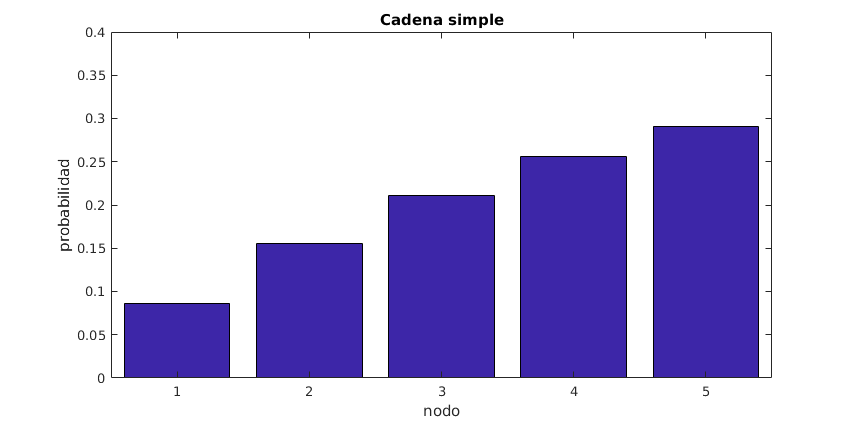
\includegraphics[width=0.7\textwidth]{img/barrascadena4.png}
	\caption{Cadena simple de nodos}
	\label{fig:Ranking cadena simple}
\end{figure}


\begin{figure}[H]
	\centering
	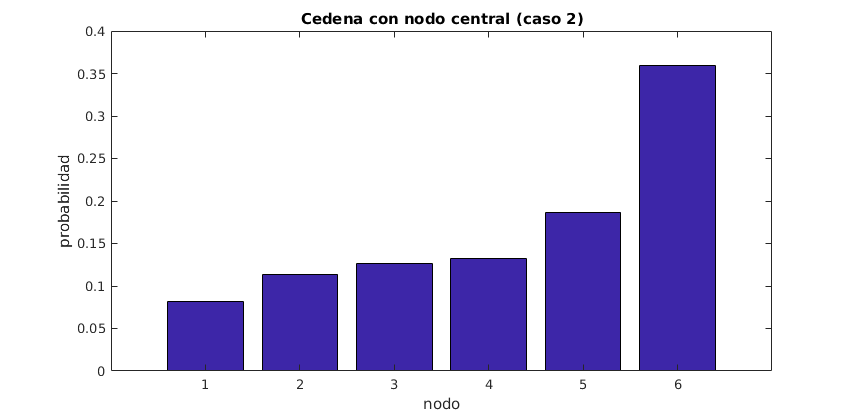
\includegraphics[width=0.7\textwidth]{img/cadena6v2.png}
	\caption{Cadena con nodo central(caso 2)}
	\label{fig:Ranking cadena con nodo central}
\end{figure}


\begin{figure}[H]
	\centering
	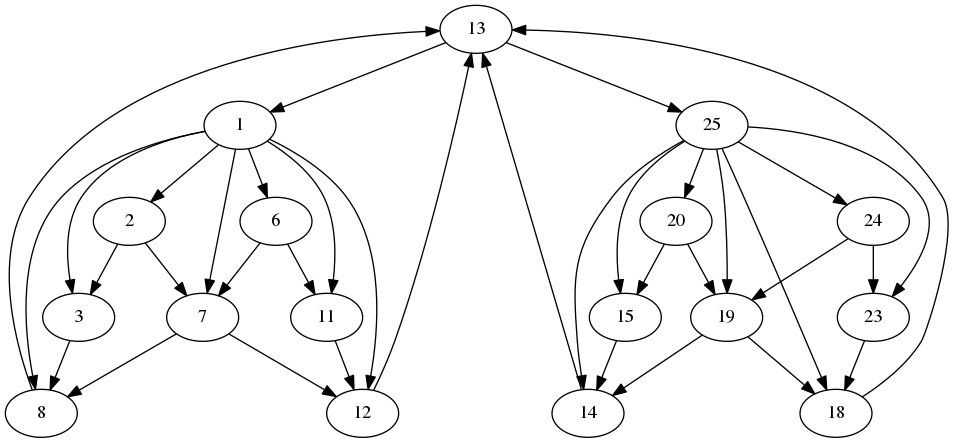
\includegraphics[width=0.7\textwidth]{img/links_salientes_25.png}
	\caption{Nodos con muchos links salientes}
	\label{fig:Ranking nodos con muchos links salientes}
\end{figure}



\begin{figure}[H]
	\centering
	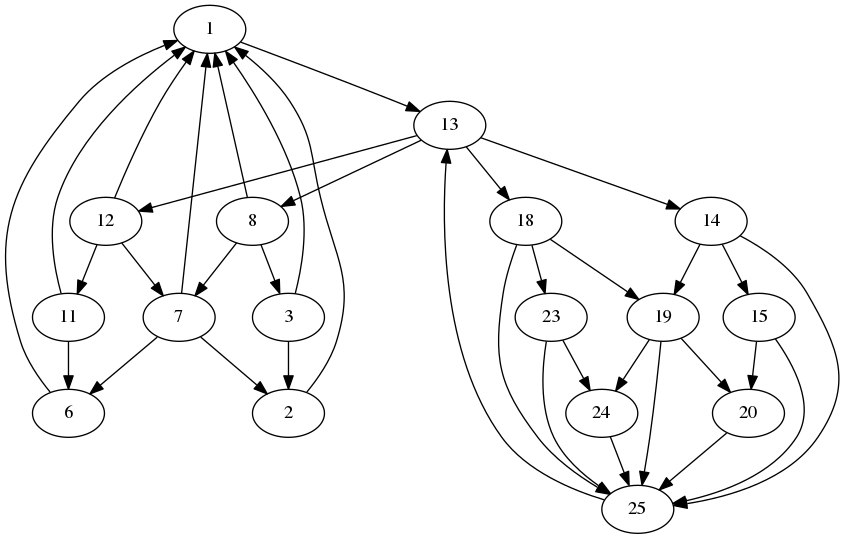
\includegraphics[width=0.7\textwidth]{img/links_entrantes_25.png}
	\caption{Nodos con muchos links entrantes}
	\label{fig:Ranking nodos con muchos links entrantes}
\end{figure}
